\subsection{定积分问题举例}
\subsubsection{曲边梯形的面积}
\paragraph{}
设$y=f(x)$在区间$[a,b]$上非负、连续。由直线$x=a, x=b, y=0$及曲线$y=f(x)$所围成的图形称为\uwave{曲边梯形},其中曲线弧称为\uwave{曲边}。矩形的高是不变的,它的面积可按公式

\begin{center}
  \text{矩形面积=高 $\times$ 底}
\end{center}
来计算。

\begin{figure}[H]
\centering
  % 曲边梯形的面积
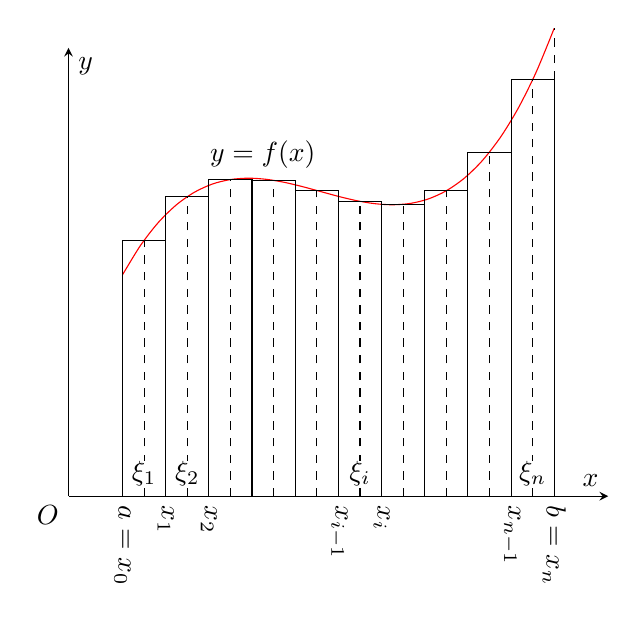
\begin{tikzpicture}[scale=1]
  \begin{axis}[clip=false,xmin=0, xmax=5,ymin=0,ymax=5, grid=none,
    xtick=\empty, ytick=\empty, axis lines=middle,
    smooth, xlabel={$x$}, ylabel={$y$}]

    % 曲线: ((x-2)**3-(x-2)**2-x)/4.0 + 4
    \addplot[draw=red,domain=0.5:4.5] {(x-2)^3/4 - (x-2)^2/4 - x/4 + 4};

    \node [above] at (1.8,3.55) {$y=f(x)$};

    \draw (0.5,0) rectangle (0.9,2.853); \draw [dashed] (0.7,0) -- (0.7,2.853);
    \draw (0.9,0) rectangle (1.3,3.34); \draw [dashed] (1.1,0) -- (1.1,3.34);
    \draw (1.3,0) rectangle (1.7,3.531); \draw [dashed] (1.5,0) -- (1.5,3.531);
    \draw (1.7,0) rectangle (2.1,3.522); \draw [dashed] (1.9,0) -- (1.9,3.522);
    \draw (2.1,0) rectangle (2.5,3.409); \draw [dashed] (2.3,0) -- (2.3,3.409);
    \draw (2.5,0) rectangle (2.9,3.288); \draw [dashed] (2.7,0) -- (2.7,3.288);
    \draw (2.9,0) rectangle (3.3,3.255); \draw [dashed] (3.1,0) -- (3.1,3.255);
    \draw (3.3,0) rectangle (3.7,3.406); \draw [dashed] (3.5,0) -- (3.5,3.406);
    \draw (3.7,0) rectangle (4.1,3.837); \draw [dashed] (3.9,0) -- (3.9,3.837);
    \draw (4.1,0) rectangle (4.5,4.644); \draw [dashed] (4.3,0) -- (4.3,4.644); \draw [dashed] (4.5,4.644) -- (4.5,5.219);

    \node [right, rotate=-90] at (0.5,0) {$a=x_0$}; \node [above,fill=white,inner sep=0.2] at (0.7,0.1) {$\xi_1$};
    \node [right, rotate=-90] at (0.9,0) {$x_1$}; \node [above,fill=white,inner sep=0.2] at (1.1,0.1) {$\xi_2$};
    \node [right, rotate=-90] at (1.3,0) {$x_2$};
    \node [right, rotate=-90] at (2.5,0) {$x_{i-1}$}; \node [above,fill=white,inner sep=0.2] at (2.7,0.1) {$\xi_i$};
    \node [right, rotate=-90] at (2.9,0) {$x_i$};
    \node [right, rotate=-90] at (4.1,0) {$x_{n-1}$}; \node [above,fill=white,inner sep=0.2] at (4.3,0.1) {$\xi_n$};
    \node [right, rotate=-90] at (4.5,0) {$b=x_n$};

    % 原点
    \node [below left] at (0,0) {$O$};
  \end{axis}
\end{tikzpicture}

  \caption{曲边梯形的面积}
  \label{曲边梯形的面积}
\end{figure}

\paragraph{}
在区间$[a,b]$中任意插入若干个分点
\begin{equation*}
  a = x_0 < x_1 < x_2 < \cdots < x_{n-1} < x_n = b,
\end{equation*}
把$[a,b]$分成$n$个小区间
\begin{equation*}
  [x_0,x_1], \; [x_1,x_2], \; \cdots, \; [x_{n-1}, x_n],
\end{equation*}
它们的长度依次为
\begin{equation*}
  \Delta x_1 = x_1 - x_0, \; \Delta x_2 = x_2 - x_1, \; \cdots, \; \Delta x_n = x_n - x_{n-1}.
\end{equation*}

\paragraph{}
因此,可求得曲边梯形面积$A$的近似值,即
\begin{align*}
  A \;\approx&\; f(\xi_1)\Delta x_1 + f(\xi_2)\Delta x_2 + \cdots + f(\xi_n)\Delta x_n \\
  =&\; \sum_{i=1}^nf(\xi_i)\Delta_i.
\end{align*}

\paragraph{}
为了保证所有小区间的长度都无限缩小,我们要求小区间长度中的最大值趋于$0$,记作$\lambda = \max|\Delta x_1, \Delta x_2, \cdots, \Delta x_n|$,则上述条件可表示为$\lambda \to 0$。当$\lambda \to 0$时(这时分段数$n$无限增多,即$n\to\infty$),取上述和式的极限,便得曲边梯形的面积

\begin{equation*}
  A = \lim_{\lambda \to 0}\sum_{i=1}^nf(\xi_i)\Delta x_i.
\end{equation*}

\subsubsection{变速直线运动的路程}
\paragraph{}
设某物体作直线运动,已知速度$v=v(t)$是时间间隔$[T_1,T_2]$上$t$的连续函数,且$v(t) \geq 0$,计算在这段时间内物体所经过的路程$s$。

\paragraph{}
对于等速直线运动,有公式
\begin{center}
  路程 = 速度 $\times$ 时间.
\end{center}

\paragraph{}
在时间间隔$[T_1,T_2]$内任意插入若干个分点
\begin{equation*}
  T_1 = t_0 < t_1 < t_2 < \cdots < t_{n-1} < t_n = T_2,
\end{equation*}
把$[T_1,T_2]$分成$n$个小时段
\begin{equation*}
  [t_0,t_1], [t_1, t_2], \cdots, [t_{n-1}, t_n],
\end{equation*}
各小时段时间的长依次为
\begin{equation*}
  \Delta t_1 = t_1 - t_0, \; \Delta t_2 = t_2 - t_1, \; \cdots, \; \Delta t_n = t_n - t_{n-1}.
\end{equation*}
相应的,在各段时间内物体经过的路程依次为
\begin{equation*}
  \Delta s_1, \Delta s_2, \cdots, \Delta s_n.
\end{equation*}
在时间间隔$[t_{i-1}, t_i]$上任取一个时刻$\tau_i \;(t_{i-1} \leq \tau_i \leq t_i)$,以$\tau_i$时的速度$v(\tau_i)$来代替$[t_{i-1}, t_i]$上各个时刻的速度,得到部分路程$\Delta s_i$的近似值,即
\begin{equation*}
  \Delta s_i \approx v(\tau_i)\Delta t_i \; (i=1,2,\cdots,n).
\end{equation*}
于是这$n$段部分路程的近似值之和就是所求变速直线运动路程$s$的近似值,即
\begin{align*}
  s \;\approx&\; v(\tau_1)\Delta t_1 + v(\tau_2)\Delta t_2 + \cdots + v(\tau_n)\Delta t_n \\
  =&\; \sum_{i=1}^nv(\tau_i)\Delta t_i.
\end{align*}
记$\lambda = \max\{\Delta t_1, \Delta t_2, \cdots, \Delta t_n\}$,当$\lambda \to 0$时,取上述和式的极限,即得变速直线运动的路程
\begin{equation*}
  s = \lim_{\lambda \to 0}\sum_{i=1}^nv(\tau_i)\Delta t_i.
\end{equation*}

\subsection{定积分定义}
\subsubsection{定义}
\paragraph{}
\textbf{定义\;}设函数$f(x)$在$[a,b]$上有界,在$[a,b]$中任意插入若干个分点
\begin{equation*}
  a = x_0 < x_1 < x_2 < \cdots < x_{n-1} < x_n = b,
\end{equation*}
把区间$[a,b]$分成$n$个小区间
\begin{equation*}
  [x_0,x_1], [x_1,x_2], \cdots, [x_{n-1},x_n],
\end{equation*}
各个小区间的长度依次为
\begin{equation*}
  \Delta x_1 = x_1 - x_0, \; \Delta x_2 = x_2 - x_1, \; \cdots, \; \Delta x_n = x_n - x_{n-1}.
\end{equation*}
在每个小区间$[x_{i-1}, x_i]$上任取一点$\xi_i \; (x_{i-1} \leq \xi_i \leq x_i)$,作函数值$f(\xi_i)$与小区间长度$\Delta x_i$的乘积$f(\xi_i)\Delta x_i \; (i=1,2,\cdots,n)$,并作出和
\begin{equation}
  S = \sum_{i=1}^n f(\xi_i)\Delta x_i,
\end{equation}
记$\lambda = \max\{\Delta x_1, \Delta x_2, \cdots, \Delta x_n\}$,如果不论对$[a,b]$怎样划分,也不论在小区间$[x_{i-1}, x_i]$上点$\xi_i$怎样选取,只要当$\lambda \to 0$时,和$S$总趋于确定的极限$I$,那么称这个极限$I$为函数$f(x)$在区间$[a,b]$上的\uwave{定积分}(简称\uwave{积分}),记作$\displaystyle\int_a^bf(x)dx$,即
\begin{equation}
  \int_a^bf(x)dx = I = \lim_{\lambda \to 0}\sum_{i=1}^nf(\xi_i)\Delta x_i,
\end{equation}
其中$f(x)$叫做\uwave{被积函数},$f(x)dx$叫做\uwave{被积表达式},$x$叫做\uwave{积分变量},$a$叫做\uwave{积分下限},$b$叫做\uwave{积分上限},$[a,b]$叫做\uwave{积分区间}。

\subsubsection{定理}
\paragraph{}
\textbf{定理1\;}设$f(x)$在区间$[a,b]$上连续,则$f(x)$在$[a,b]$上可积。

\paragraph{}
\textbf{定理2\;}设$f(x)$在区间$[a,b]$上有界,且只有有限个间断点,则$f(x)$在$[a,b]$上可积。

\subsection{定积分的近似计算}
\subsubsection{矩形法}
\paragraph{}
参考图\figureref{曲边梯形的面积},近似计算公式:
\begin{equation}
  \int_a^bf(x)dx \approx \frac{b-a}{n}(y_1+y_2+\cdots+y_n).
\end{equation}

\subsubsection{梯形法}
\paragraph{}
原理:将曲线$y=f(x)$上的小弧段$\overarc{M_{i-1}M_i}$用直线段$\overline{M_{i-1}M_i}$代替,然后用梯形代替要求的面积,由此得到定积分的近似值为
\begin{align}
\begin{split}
  \int_a^bf(x)dx \;\approx&\; \frac{b-a}{n}\big(\frac{y_0+y_1}{2} + \frac{y_1+y_2}{2} + \cdots + \frac{y_{n-1}+y_n}{2}\big) \\
  =&\; \frac{b-a}{n}\big(\frac{y_0+y_n}{2}+y_1 + y_2 + \cdots + y_{n-1}\big)
\end{split}
\end{align}

\begin{figure}[H]
\centering
  % 梯形法
\begin{tikzpicture}[scale=0.8]
  \begin{axis}[clip=false,xmin=0, xmax=5.5,ymin=0,ymax=5.5, grid=none,
    xtick=\empty, ytick=\empty, axis lines=middle,
    smooth, xlabel={$x$}, ylabel={$y$}]

    % 曲线
    \addplot[draw=red,domain=1:4.5] {0.3*sin(deg(2*x-3)) + 3.5};

    \draw [pattern=north east lines] (2.2,0) -- (2.2,3.796) -- (3.2,3.423) -- (3.2,0) -- (2.2,0);

    \node [below] at (2.2,0) {$x_{i-1}$};
    \node [left] at (2.2,1.9) {$y_{i-1}$};
    \node [above] at (2.2,3.796) {$M_{i-1}$};

    \node [below] at (3.2,0) {$x_i$};
    \node [right] at (3.2,1.9) {$y_i$};
    \node [above] at (3.2,3.423) {$M_i$};

    \node [below] at (4.2,3.268) {$y=f(x)$};

    % 原点
    \node [below left] at (0,0) {$O$};
  \end{axis}
\end{tikzpicture}

  \caption{梯形法}
  \label{梯形法}
\end{figure}

\subsubsection{抛物线法(辛普森法)}
\paragraph{}
原理:将曲线$y=f(x)$上的两个小弧段$\overarc{M_{i-1}M_i}$和$\overarc{M_iM_{i+1}}$合并起来,用过$M_{i-1}, M_i, M_{i+1}$三点的抛物线$y = px^2+qx+r$代替。经推导得,此抛物线弧段为曲边、以$[x_{i-1},x_{i+1}]$为底的曲边梯形面积为
\begin{equation}
  \frac{1}{6}(y_{i-1}+4y_i+y_{i+1}) \bigcdot 2\Delta x = \frac{b-a}{3n}(y_{i-1} + 4y_i + y_{i+1}).
\end{equation}
取$n$为偶数,得到定积分的近似值为
\begin{align}
\begin{split}
  \int_a^bf(x)dx \;\approx&\; \frac{b-a}{3n}[(y_0+4y_1+y_2) + (y_2+4y_3+y_4) + \cdots + (y_{n-2}+4y_{n-1}+y_n)] \\
  =&\; \frac{b-a}{3n}[y_0+y_n+4(y_1+y_3+\cdots+y_{n-1}) + 2(y_2+y_4+\cdots+y_{n-2})].
\end{split}
\end{align}

\begin{figure}[H]
\centering
  % 抛物线法
\begin{tikzpicture}[scale=0.8]
  \begin{axis}[clip=false,xmin=0, xmax=6,ymin=0,ymax=6, grid=none,
    xtick=\empty, ytick=\empty, axis lines=middle,
    smooth, xlabel={$x$}, ylabel={$y$}]

    % 曲线
    \addplot[draw=red,domain=1:5] {0.3*sin(deg(2*x-2)) + x^2/20 + 3};

    \draw (2.5,0) -- (2.5,3.355);
    \draw (3.25,0) -- (3.25,3.235);
    \draw (4,0) -- (4,3.72);

    \addplot[draw=blue,domain=1.7:4.8] {0.539*x^2 -3.26*x + 8.136};
    \addplot[domain=2.5:4,pattern=north east lines,draw opacity=0] {0.539*x^2 -3.26*x + 8.136} \closedcycle;

    \draw [fill] (2.5,3.355) circle [radius=0.03];
    \draw [fill] (3.25,3.235) circle [radius=0.03];
    \draw [fill] (4,3.72) circle [radius=0.03];

    \node [below] at (2.5,0) {$x_{i-1}$};
    \node [above] at (2.5,3.355) {$M_{i-1}$};

    \node [below] at (3.25,0) {$x_i$};
    \node [above] at (3.25,3.235) {$M_i$};

    \node [below] at (4,0) {$x_{i+1}$};
    \node [above,rotate=45] at (4,3.72) {$M_{i+1}$};

    \node [below] at (5,4.21) {$y=f(x)$};

    % 原点
    \node [below left] at (0,0) {$O$};
  \end{axis}
\end{tikzpicture}

  \caption{抛物线法}
  \label{抛物线法}
\end{figure}

\subsection{定积分的性质}
\paragraph{}
补充
\begin{enumerate}
  \item 当$a=b$时,$\displaystyle\int_a^bf(x)dx=0$;
  \item 当$a>b$时,$\displaystyle\int_a^bf(x)dx = -\int_b^af(x)dx$。
\end{enumerate}

\paragraph{}
\textbf{性质1\;}$\displaystyle\int_a^b[f(x)\pm g(x)]dx = \int_a^bf(x)dx \pm \int_a^bg(x)dx$。

\paragraph{}
\textbf{性质2\;}$\displaystyle\int_a^bkf(x)dx = k\int_a^bf(x)dx$($k$是常数)。

\paragraph{}
\textbf{性质3\;}设$a<c<b$,则积分区间具有\uwave{可加性}
\begin{equation}
  \int_a^bf(x)dx = \int_a^cf(x)dx + \int_c^bf(x)dx.
\end{equation}

\paragraph{}
\textbf{性质4\;}如果在区间$[a,b]$上$f(x)\equiv 1$,则
\begin{equation}
  \int_a^b1dx = \int_a^bdx=b-a.
\end{equation}

\paragraph{}
\textbf{性质5\;}如果在区间$[a,b]$上,$f(x)\geq 0$,则
\begin{equation}
  \int_a^bf(x)dx \geq 0 \; (a<b).
\end{equation}

\paragraph{}
\textbf{推论1\;}如果在区间$[a,b]$上,$f(x)\leq g(x)$,则
\begin{equation}
  \int_a^bf(x)dx \leq \int_a^bg(x)dx \; (a<b).
\end{equation}

\paragraph{}
\textbf{推论2\;}$\displaystyle\big| \int_a^bf(x)dx \big| \leq \int_a^b|f(x)|dx \; (a<b)$。

\paragraph{}
\textbf{性质6\;}设$M$及$m$分别是函数$f(x)$在区间$[a,b]$上的最大值及最小值,则
\begin{equation}
  m(b-a) \leq \int_a^bf(x)dx \leq M(b-a) \; (a<b).
\end{equation}

\paragraph{}
\textbf{性质7(定积分中值定理)\;}如果函数$f(x)$在积分区间$[a,b]$上连续,则在$[a,b]$上至少存在一个点$\xi$,使下式成立:
\begin{equation}
  \int_a^bf(x)dx = f(\xi)(b-a) \; (a\leq\xi\leq b).
\end{equation}
这个公式叫做\uwave{积分中值公式}。

\begin{figure}[H]
\centering
  % 定积分中值定理示例
\begin{tikzpicture}[scale=0.8]
  \begin{axis}[clip=false,xmin=0, xmax=6,ymin=0,ymax=6, grid=none,
    xtick=\empty, ytick=\empty, axis lines=middle,
    smooth, xlabel={$x$}, ylabel={$y$}]

    \addplot[draw=red,domain=1:5] {2*ln(x) + 2};

    \node [above] at (4,5.22) {$y=f(x)$};

    \draw (1,0) -- (1,2);
    \draw (5,0) -- (5,5.22);
    \draw [dashed] (3,0) -- (3,4.2);
    \draw [dashed] (0,4.2) -- (5,4.2);
    \draw [dashed] (1,0) -- (1,4.2);

    \node [below] at (1,0) {$a$};
    \node [below] at (3,0) {$\xi$};
    \node [below] at (5,0) {$b$};
    \node [left] at (0,4.2) {$f(\xi)$};

    % 原点
    \node [below left] at (0,0) {$O$};
  \end{axis}
\end{tikzpicture}

  \caption{定积分中值定理示例}
  \label{定积分中值定理示例}
\end{figure}

\paragraph{}
按积分中值公式所得函数$f(x)$在区间$[a,b]$上的\uwave{平均值}:
\begin{equation}
  f(\xi) = \frac{1}{b-a}\int_a^bf(x)dx.
\end{equation}
